\documentclass[a4paper,10pt,oneside]{report}%pridat twoside, do [] pre obojstrannu tlac
\pagestyle{headings}
\usepackage[top=2.5cm, bottom=2.5cm, left=3.5cm, right=2cm]{geometry} %odporucane okraje
\linespread{1.50}

%% Generally used
\usepackage{ebproof}
\usepackage{amsthm}
\usepackage{amsmath}
\usepackage{amssymb, upgreek}
\usepackage{mathtools}
\usepackage{color}
\usepackage[T1]{fontenc}
%% Generally used

%% Lean specific
\usepackage[utf8x]{inputenc}
\definecolor{keywordcolor}{rgb}{0.7, 0.1, 0.1}   % red
\definecolor{commentcolor}{rgb}{0.4, 0.4, 0.4}   % grey
\definecolor{symbolcolor}{rgb}{0.0, 0.1, 0.6}    % blue
\definecolor{sortcolor}{rgb}{0.1, 0.5, 0.1}      % green
\definecolor{errorcolor}{rgb}{1, 0, 0}           % bright red
\definecolor{stringcolor}{rgb}{0.5, 0.3, 0.2}    % brown
\usepackage{pict2e,picture}

\usepackage{listings}
\def\lstlanguagefiles{lstlean.tex}
\lstset{language=lean}
%% Lean specific

%% Covering

\newcommand{\coveringA}{%
  \mathrel{-\mkern-4mu}<%
}
\newcommand{\coveringB}{\mathrel{\text{$\vcenter{\hbox{\pictcoveringB}}$}}}

\newcommand{\pictcoveringB}{%
  \begin{picture}(1em,.5em)
  \roundcap
  \put(0,.25em){\line(1,0){.6em}}
  \put(.6em,.25em){\line(3,1){.4em}}
  \put(.6em,.25em){\line(3,-1){.4em}}
  \end{picture}%
}
%% Covering

%% Powerset
\newcommand{\powerset}{\raisebox{.15\baselineskip}{\Large\ensuremath{\wp}}}
%% Powerset
\newcommand{\nothing}{\varnothing}

\newtheorem{theorem}{Theorem}


\author{Mat\'u\v{s} Behun}
\title{Lattice theory notes}

\begin{document}

\tableofcontents

\section{Úvod}

%Pri procese rozširovania matematickej teórie vytvárame tvrdenia generalizujúce jej princípy.
%Ak chceme aby náša teória bola správna, všetky jej tvrdenia musia byť logicky odvodené z postulátov alebo tvrdení z nich odvodených.
%Potvrdenie správnosti tvrdenia, vyslovením predpokladu, axiómu alebo napísaním formule ktorú dostaneme aplikáciou dedukčného pravidla na niektoré v postupnosti predchádzajúce formule nazývame dôkazom.

%% Je to pravda?
%Z kvalitatívneho hľadiska pri vyslovení dôkazu uvažujeme o všeobecnosti dôkazu a správnosti aplikácie dedukčného pravidla.
%% Je to vhodný príklad(chcel som uviest priklad na prvy pohlad spravneho tvrdenia ktore bolo dokazane ako nespravne ? Ako správne citovať? Nápad som mal odtiaľto https://en.wikipedia.org/wiki/List_of_disproved_mathematical_ideas
%O nutnosti korektného dokazovania tvrdení hovorí napríklad tvrdenie z teórie čísel o hornom ohraničení počtu prvočísel logaritmickým integrálom.

%\begin{equation}
    %\pi(x) \leq \int_{0}^{x} \frac{1}{ \ln{t} } dt
%\end{equation}

%Tvrdenie bolo považované za správne Bernhardom Riemannom a evidencia to taktiež naznačovala.
%Neskôr sa ukázalo že tvrdenie nie je správne pri čísle pod hodnotou $10^{317}$.
%% Doplniť rok
%Veta o 4 farbách ktorá bola vyslovená v roku 1852 Francisom Guthrie ktorá hovorí, že každá rovinná mapa je zafarbiteľná 4 farbami.
%% 18-faces
%Táto veta bola nesprávne dokázaná v roku Kempom (1879) and Taitom (1880). Kempov dôkaz bol vyvrátený o 10 rokov mapov s 18 stenami.
%% Je lepšie skloňovať cudzie mená?
%Pri dôkaze tejto vety bol neskôr v roku 1977 Appelom and Hakenom z časti využitý počítač pre kontrolu špeciálnych diskrétnych prípadov.


\chapter{Curry-Howardov izomorfizmus}

\section{Formalizovanie dôkazu}

Dôkaz z teórie usporiadania. Tak ako je Program = Proof

Otázka ohľadne konzistentnosti dôkazu.

\section{Prirodzená dedukcia}

% Formula vyrokoveho poctu
\begin{theorem}[Výroková premenná, formula]
    Majme spočítateľnú množinu $\mathcal{X}$ výrokových premenných. Množina výrokov
    alebo formúl $\mathcal{A}$ generovanú nasledovnou gramatikou:
    \begin{equation}
        A, B ::= X | A \implies B | A \wedge B | A \vee B | \neg A | \top | \bot
    \end{equation}
    Kde $X \in \mathcal{X}$ reprezentuje výrokovú premennú, a $A, B \in \mathcal{A}$
    výrok.
\end{theorem}

V prípade nasledovného výroku je precedencia $\neg$ vyššia ako $\vee$ alebo $\wedge$
a tá je vyššia ako $\implies$. Binárne operátory sú asociatívne sprava.

\begin{align*}
    \neg A \wedge B \wedge C &\implies A \vee B \\
    (\neg A \wedge (B \wedge C)) &\implies (A \vee B) \\
\end{align*}

\begin{theorem}
    Kontextom(systém predpokladov) rozuemieme zoznam výrokov značených
    \begin{equation}
        \Gamma = P_{1}, \dots , P_{n}
    \end{equation}
    Dedukciou nazývame dvojicu pozostávajúcu z kontextu a výroku.
    \begin{equation}
        \Gamma \vdash A
    \end{equation}
\end{theorem}

Výraz čítame ako $A$ je možné dokázať zo systému predpokladov $\Gamma$.

\begin{theorem}
    Dedukčné pravidlo pozostáva z množiny dedukcií $\Gamma_{i}$ ktoré nazývame
    prepokladom. Dolnú časť dedukčného pravidla $\Gamma$ nazývame záverom.
    \begin{equation}
        \begin{prooftree}
            \hypo{\Gamma_{1} \vdash A_{1}}
            \hypo{\dots}
            \hypo{\Gamma_{n} \vdash A_{n}}
            \infer3[]{\Gamma \vdash A}
        \end{prooftree}
    \end{equation}
\end{theorem}
Pravidlá prirodzenej intuicionistickej logiky:
\begin{center}
    \begin{prooftree}
        \infer0[(ax)]{\Gamma,A,\Gamma' \vdash: A}
    \end{prooftree}
\end{center}
\vskip 0.2in
\begin{minipage}[t]{0.48\textwidth}
    \begin{prooftree}
        \hypo{\Gamma \vdash A \implies B}
        \hypo{\Gamma \vdash A}
        \infer2[$(\implies_{E})$]{\Gamma : B}
    \end{prooftree}
\end{minipage}
\hfill
\begin{minipage}[t]{0.48\textwidth}
    \begin{prooftree}
        \hypo{\Gamma, A \vdash B}
        \infer1[$\implies_{I}$]{\Gamma : B}
    \end{prooftree}
\end{minipage}
\vskip 0.2in
\begin{minipage}[t]{0.48\textwidth}
    \begin{prooftree}
        \hypo{\Gamma, A \vdash B}
        \infer1[$(\wedge^{l}_{E})$]{\Gamma : A}
    \end{prooftree}
    \begin{prooftree}
        \hypo{\Gamma, A \vdash B}
        \infer1[$(\wedge^{r}_{E})$]{\Gamma : B}
    \end{prooftree}
\end{minipage}
\hfill
\begin{minipage}[t]{0.48\textwidth}
    \begin{prooftree}
        \hypo{\Gamma \vdash A}
        \hypo{\Gamma \vdash B}
        \infer2[$(\wedge_{I})$]{\Gamma \vdash A \wedge B}
    \end{prooftree}
\end{minipage}
\vskip 0.2in
\begin{minipage}[t]{0.48\textwidth}
    \begin{prooftree}
        \hypo{\Gamma \vdash A \vee B}
        \hypo{\Gamma, A \vdash C}
        \hypo{\Gamma, B \vdash C}
        \infer3[$(\vee_{E})$]{\Gamma \vdash C}
    \end{prooftree}
\end{minipage}
\hfill
\begin{minipage}[t]{0.48\textwidth}
    \begin{prooftree}
        \hypo{\Gamma \vdash B}
        \infer1[$(\vee_{I}^{r})$]{\Gamma \vdash A \vee B}
    \end{prooftree}
    \begin{prooftree}
        \hypo{\Gamma \vdash A}
        \infer1[$(\vee_{I}^{l})$]{\Gamma \vdash A \vee B}
    \end{prooftree}
\end{minipage}
\vskip 0.2in
\begin{minipage}[t]{0.48\textwidth}
    \begin{prooftree}
        \hypo{\Gamma \vdash \neg A}
        \hypo{\Gamma \vdash A}
        \infer2[$(\neg_{E})$]{\Gamma \vdash \bot}
    \end{prooftree}
\end{minipage}
\hfill
\begin{minipage}[t]{0.48\textwidth}
    \begin{prooftree}
        \hypo{\Gamma, A \vdash \bot}
        \hypo{\Gamma \vdash A}
        \infer2[$(\neg_{I})$]{\Gamma \vdash \neg A}
    \end{prooftree}
\end{minipage}
\vskip 0.2in
\begin{center}
    \begin{prooftree}
        \hypo{\Gamma \vdash \bot}
        \infer1[$(\bot_{E})$]{\Gamma \vdash A}
    \end{prooftree}
\end{center}

V prípade že tieto pravidlá čítame zhora nadol hovoríme o dedukcii.
Ak čítame pravidlá zdola nahor hovoríme o indukčnom spôsobe.

\begin{theorem}
    Fragmentom intuionistickej logiky nazývame, systém ktorý dostaneme ak ho obmedzíme
        len na niektoré z predchádzajúcich pravidiel.
\end{theorem}

\begin{theorem}
    Implikačným fragmentom intuionistickej logiky dostaneme v prípade ak formuly
        budú tvorené gramatikou
    \begin{equation}
        A,B ::= X | A \implies B
    \end{equation}
    a pravidlami (ax), ($\implies_{E}$), ($\implies_{I}$)
\end{theorem}

% TODO spravit priklad
% (𝐴∧𝐵)→((𝐴→𝐶)→¬(𝐵→¬𝐶))

V prípade že chceme aby výrokove formuly korenšpondovali s typmi ktoré su prezentované neskôr.
Ich booleova reprezentácia s hodnotami $1,0$ je nahradená otázkou existencie prvkov v množine.
V prípade implikácie o existencii funkcie v množine.
Funkcie v programoch ale môžu mať pri rovnakých vstupoch a výstupoch mať rôznu výpočtovú zložitosť.
Dôvod prečo by sme sa mali pozerať na dôkazy(podľa publikácie Gir11) v troch rovinách.

\begin{itemize}
    \item 1. Booleovský - tvrdenia sú booleovské hodnoty, zaujímame sa o dokázateľnosť tvrdenia
    \item 2. Existenčný - tvrdenia sú množiny, aké funkcie môžu byť
    \item 3. Úmyselný/Zámerový(Intentional) - zaujímame sa o zložitosť vytvoreného dôkazu a ako sa zjednoduší cez (cut eliminitation)
\end{itemize}

\subsection{Intuicionizmus}

Jedným zo smerov matematickej filozofie týkajucej sa rozvoja teórie je konštruktivizmus.
Konštruktivizmus hovorí o potrebe nájsť alebo zostrojiť matematický objekt k tomu
    aby bola dokázaná jeho existencia.
Jeden z motivačných príkladov takéhoto prístupu je možnosť dokázania pravdivosti
výroku $p \vee \neg p$ cez dôkaz sporom $\neg p$ ktorý nehovorí ako zostrojiť objekt
$p$ len o jeho existencii.
Tento smer tvorí viacero "škôl" okrem iných finitizmus, predikativizmus, intuicionizmus.
Intuitionizmus je teda konštruktívny prístup k matematike v duchu
    Brouwera(1881-1966) a Heytinga(1898-1980).
Filozofickým základom tochto prístupu princíp že matematika je výtvorom mentálnej
činnosti a nepozostáva z výsledkov  formálnej manipulácie symbolov ktoré sú iba
sekundárne.
Jedným z princípov intuicionizmus je odmietnutie tvrdenia postulátu klasickej
logiky a to zákona vylúčenia tretieho.

\begin{equation}
    p \vee \neg p
\end{equation}

Dôvodom je z konštruktívneho pohľadu nezmyselnosť uvažovania nad pravdivosťou
    výroku nezávisle od uvažovaného tvrdenia.
Výrok je teda pravdivý ak existuje dôkaz o jeho pravidovsti a nepravdivé
    ak existuje dôkaz ktorý vedie k sporu.

\begin{itemize}
    \item konjukcii $ p \wedge q $ ako o výroku hovoriacom o existencii dôkazov $p$ a zároveň $q$,
    \item disjunkcii $ p \wedge q $ ako existencii konštrukcii dôkazu jedného z výrokov $p, q$,
    \item $ p \implies q $ je metóda(funkcia) transformácie každej konštrukcie $p$ k dôkazu $q$,
    \item neexistencie dôkazu nepravdivého tvrdenia, iba dôkazu ktorý vedie k sporu $p \implies \bot$
    \item konštrukcia $\neg p$ je metóda ktorá vytvorí každú konštrukciu $p$ na neexistujúci objekt
\end{itemize}

konjukcii $ A \wedge B $ ako $ A \times B $
$ A \vee B $ ako $ A \sqcup B $ disjunktne zjednotenie
$ \neg A = A \implies \perp $ existencie kontrapríkladu

\section{Lambda kalkulus}

\begin{theorem}
    Majme nekonečnú množinu $ \mathcal{X}={x,y,z,\dots}$ ktorých elementy nazývame premenné.
Množinu $\Lambda$ tvorenú $\lambda$-termínmy je potom generovaná nasledovnou gramatikou:
    \begin{equation}
        t, u ::= x | t u | \lambda x.t
    \end{equation}
\end{theorem}
\noindent Význam jednotlivých termínov je
\begin{align*}
     x          & \textrm{ - je premennou }\\
     t u        & \textrm{ - je aplikáciou termínu $t$ s argumentom $u$ }\\
    \lambda x.t & \textrm{ - je abstrakciou $t$ nad $x$ }
\end{align*}
Príklady lambda termínov:

\begin{align*}
    & t x \\
    & (\lambda y . \lambda x . t y )) \\
    & (\lambda y.y x) (\lambda x . x) \\
    & t u v = ( t u ) v
\end{align*}

Aplikácia $\lambda$-termínov je implicitne aplikovaná zľava.

Pri výraze
\begin{equation}
    \lambda x . t x = \lambda x . (t x)
\end{equation}
je precedencia aplikácie vyššia ako abstrakcia.

A abstrakciu s troma argumentmi je možné prepísať do troch po sebe nasledujúcich.
\begin{equation}
    \lambda x y z . t = \lambda x . \lambda y . \lambda z . t
\end{equation}

\begin{theorem}
    Premenná x sa vo výraze
    \begin{equation}
        \lambda x . t
    \end{equation}
    abstrakciou viaže na termín $t$. O premennej $x$ hovoríme že je viazaná.
    O premenných ktoré nie sú viazané sú voľné.
    \begin{align*}
        VP(x) &= {x} \\
        VP(\lambda x.t) &= VP(t)  \setminus \{x\} \\
        VP(t v) &= VP(t) \cup VP(v)
    \end{align*}
\end{theorem}

\begin{theorem}
    Premenovaním nazývame nahradenie voľných premenných v termíne.
    \begin{equation}
        t \{ y / x \}
    \end{equation}
\end{theorem}
V termíne $t$ je premenovaná premenná $x$ za $y$.

% TODO pridaj priklady
\subsection{$\alpha$-ekvivalencia}
\begin{theorem}
    O výrazov hovoríme že sú alfa-ekvivalentné ak sa výrazy rovnajú až na premenovanie.
\end{theorem}

\begin{theorem}
    O substutícii hovoríme pri nahradení jednej premenej druhou.
    \begin{equation}
        t [ y / x ]
    \end{equation}
\end{theorem}

Nahradenie je silnejšie a vieme nahradiť aj premmenné viazanné abstrakciou.

\subsection{$\beta$-ekvivalencia}

\begin{minipage}[t]{0.48\textwidth}
    \begin{prooftree}
        \infer0[($\beta_{s}$)]{(\lambda x.t)u \to_{\beta} t [ u / x ]}
    \end{prooftree}
\end{minipage}
\hfill
\begin{minipage}[t]{0.48\textwidth}
    \begin{prooftree}
        \hypo{t \to_{\beta} t'}
        \infer1[($\beta_{\lambda}$)]{(\lambda x.t)u \rightarrow_{\beta} t [ u / x ]}
    \end{prooftree}
\end{minipage}
\vskip 0.2in
\begin{minipage}[t]{0.48\textwidth}
    \begin{prooftree}
        \hypo{t \to_{\beta} t'}
        \infer1[($\beta_{l}$)]{t u \rightarrow_{\beta} t' u}
    \end{prooftree}
\end{minipage}
\hfill
\begin{minipage}[t]{0.48\textwidth}
    \begin{prooftree}
        \hypo{u \to_{\beta} u'}
        \infer1[($\beta_{r}$)]{t u \rightarrow_{\beta} t u'}
    \end{prooftree}
\end{minipage}
\vskip 0.2in

% TODO vymysliet iny strom, tento je prevzaty
\begin{equation}
    \begin{prooftree}
        \infer0[($\beta_{s}$)]{(\lambda y.y)x \to_{\beta} x}
        \infer1[($\beta_{l}$)]{(\lambda y.y)xz \to_{\beta} xz}
        \infer1[($\beta_{\alpha}$)]{\lambda x.(\lambda y.y)xz \to_{\beta} \lambda x . xz}
    \end{prooftree}
\end{equation}

\begin{theorem}
    Definujme rekurziu volania funkcie nasledovne
    \begin{align}
        f^{0}x &= x \\
        f^{n}x &= f(f^{n-1}x) \\
    \end{align}
    Potom Churchove číslo $c_{n}$ je $\lambda$-termín
    \begin{equation}
        c_{n} = \lambda s . \lambda z . s^{n} (z)
    \end{equation}
\end{theorem}

Prirodzené čísla je potom definovať
\begin{align*}
    0 &= \lambda f x . x \\
    1 &= \lambda f x . f x \\
    1 &= \lambda f x . f (f x) \\
    2 &= \lambda f x . f ( f (f x))
\end{align*}

\begin{align*}
    succ(n) &=           (\lambda n f x .  f( n f x ))(\lambda f x . f^{n} x) \\
           &\to_{\beta} \lambda f x . f (( \lambda f x . f^{n} x ) f x)      \\
           &\to_{\beta} \lambda f x . f (( \lambda x . f^{n} x) x)           \\
           &\to_{\beta} \lambda f x . f (f^{n} x)                            \\
           &=           \lambda f x . f^{n+1} x                              \\
           &= n + 1
\end{align*}

Operáciu sčítania je potom možné definovať vykonať
\begin{theorem}
    $f_{+} = \lambda x. \lambda y. \lambda s. \lambda z. x s (y s z)$
\end{theorem}

Podobným spôsobom môžeme vytvoriť 
\begin{theorem}
    \begin{align*}
        True &= \lambda x y . x \\
        False &= \lambda x y . y
    \end{align*}
\end{theorem}

\begin{align*}
    if = \lambda b x y . b x y
\end{align*}

\begin{align*}
    if \textrm{ True } t u = (\lambda bxy.bxy)(\lambda xy.x) tu & \to_{\beta} (\lambda xy.(\lambda xy.x)xy)tu \\
                                                     & \to_{\beta} (\lambda y.( \lambda xy.x)ty)u \\
                                                     & \to_{\beta} (\lambda xy.x)tu \\
                                                     & \to_{\beta} (\lambda y.t)u \\
                                                     & \to_{\beta} t
\end{align*}

\begin{theorem}
    Jednoduchý $\lambda$ kalkulus je ekvivalentný výpočtovej sile turingovho stroja.
    Bez dôkazu
\end{theorem}

\section{Typovo jednoduchý $\lambda$-calculus}

Typový lambda calculus je rozšírením jednoduchého o typy

\begin{theorem}
    Majme množinu $U$ spočítateľnú nekonečnú abecedu obsahujúcu typové premenné.
    Potom množina $\Pi$ obsahuje reťazce jednoduchých typov ktoré su generované
    gramatikov:
    \begin{equation}
        \Pi ::= U | (\Pi \to \Pi)
    \end{equation}
\end{theorem}

\begin{theorem}
    Kontextom rozumieme množinu $C$ tvoriacu 
    \begin{equation}
        { x_{1} : \tau_{1}, \dots, x_{n} : \tau_{n} }
    \end{equation}
    kde $\tau_{1}, \dots, \tau_{n} \in \Pi$ a $x_{1}, \dots , x_{n} \in$
    Koobor kontextu je množina obsahujúca
    \begin{equation}
        domain(\Gamma) = { x_{1}, \dots, x_{n} }
    \end{equation}
    Oboor kontextu je množina obsahujúca
    \begin{equation}
        range( \Gamma ) = { \tau \in \Pi  | (x : \tau ) \in \Gamma }
    \end{equation}
\end{theorem}

\noindent Príklady generované gramatikou
\begin{itemize}
    \item $\vdash \lambda x.x : \sigma \to \sigma$
    \item $\vdash \lambda x. \lambda y.x : \sigma \to \tau \to \sigma$
    \item $\vdash \lambda x. \lambda y. \lambda z.x z (y z): (\sigma \to \tau \to \rho) \to (\rho \to \tau) \to \sigma \to \rho$
\end{itemize}

\begin{theorem}
    Postupnosť je trojica značená
    \begin{equation}
        \Gamma \vdash t : A
    \end{equation}
tvorená kontextom $\Gamma$, $\lambda$-termínom $t$ a typom $A$.
\end{theorem}

Termín $t$ je typu $A$ ak v kontexte $\Gamma$ ak je postupnosť derivovateľná pomocou pravidiel:
\begin{itemize}
    \item ax: v kontexte $x$ je typu $A$
    \item $\overset{I}{\rightarrow}$: ak je $x$ typu $A$, $t$ je typu B, potom
        funkcia $\lambda x.t$ ktorá asociuje $x$ $t$ je typu $A \to B$
    \item $\overset{E}{\rightarrow}$: daná je funkcia $t$ je typu $A \to B$
        a argument $u$ je typu $A$, vysledok aplikácia $t u$ je typu $B$
\end{itemize}

\begin{center}
    \begin{prooftree}
        \infer0[ax]{\Gamma \vdash x : \Gamma(x)}
    \end{prooftree}
\end{center}
\vskip 0.2in
\begin{minipage}[t]{0.48\textwidth}
    \begin{prooftree}
        \hypo{\Gamma , x : A \vdash t : B }
        \infer1[$\overset{I}{\rightarrow}$]{\Gamma \lambda x^{A}.t : A \to B}
    \end{prooftree}
\end{minipage}
\hfill
\begin{minipage}[t]{0.48\textwidth}
    \begin{prooftree}
        \hypo{\Gamma \vdash t : A \to B }
        \hypo{\Gamma \vdash u : A }
        \infer2[$\overset{E}{\rightarrow}$]{\Gamma \vdash t u : B}
    \end{prooftree}
\end{minipage}

\section{Curry-Howardov izomorfizmus}

\begin{center}
    \begin{tabular}{ c c }
        Intuinistická logika & Typovo jednoduchý $\lambda$ kalkulus \\
        \hline
        termín                  & dôkaz \\
        typová premenná         & propozičná premenná \\
    \end{tabular}
\end{center}

\begin{theorem}{Curry-Howard isomorphism}
    \begin{itemize}
        \item If $\Gamma \vdash M : \varphi \textrm{ potom } |\Gamma|  \vdash \varphi.$
        \item If $\Gamma \vdash \varphi \textrm{ potom existuje } M \in \Lambda_{\Pi}
            \textrm{ také že } \Delta \vdash M : \varphi, \textrm{ kde }
            \Delta = { ( x_{\varphi} : \varphi ) | \varphi \in \Gamma }$
    \end{itemize}
\end{theorem}

\section{Počítačom asistované dokazovanie}
    To com som vravel v prezentacii, historia, na zaciatku sa pouzivalo
\chapter{Lean dokazovací asistent}
    Lean je dokazovací asistent ktorý bol vytvorený otvorený softvérový projekt
Leonardom de Mourom v Microsoft Reasearch v roku 2013.
    Jazyk sa neustále vyvýja a momentálne sa nachádza vo štvrtej iterácii \cite{lean4} zatiaľ čo komunitný projekt matematickej knižnice mathlib sa stále vyvíja v tretej verzii\cite{lean3} vyvýjanej od roku 2017.
    Implementácia Lean-u je v jazyku C++ a jeho jadro má 8000 riadkov.
    Prostredie je dostupné pre operačné systémy Linux, Windows a Darwin.
    Interaktívne prostredie pre dokazovanie je podporované pre editory \emph{Emacs} a \emph{Visual Studio Code}.

    Lean podobne ako \emph{Coq} je založené na kalkule konštrukcií ktorý je zovšeobecnením teórie jednoduchých typov
    a teórii závislostných typov.
\section{Mathlib}
    % zdruzovat mozem vcelarov
    Mathlib je komunitný projekt\cite{mathlib} ktorého cieľom je združovať matematickú
teóriu implementovanú v Lean-e.
    Do projektu je možné jednoducho prispievať po udelení privilégií niektorým zo
správcov repozitára a odobrením požiadavky na začlenenie kódu.
    Väčšina obsahu mathlibu obsahuje matematiku na vysokoškolskej úrovni.
    V dobre písania práce je najvyššia hierarchia teórie nasledovná:
\begin{lstlisting}
algebra/
category_theory/
data/
geometry/
measure_theory/
probability_theory/
algebraic_geometry/
combinatorics/
group_theory/
representation_theory/
algebraic_topology/
computability/
dynamics/
linear_algebra/
number_theory/
ring_theory/
analysis/
control/
field_theory/
logic/
order/
set_theory/
topology/
\end{lstlisting}
    V kontraste s inými modernými dokazovacími asistentami má mathlib množstvo
prispievateľov akademické vzdelanie v čistej matematike\cite{mathlib_paper} čo
ovplyvnilo aj jeho obsah.

\section{Vývojové prostredie}
    V našom prípade sme pracovali vo vývojovom prostredí \emph{Visual studio code}
v kombinácií s jeho leanovským rozšírením ktoré je možné nainštalovať cez
\emph{marketplace} Prostredie sa skladá z editora podporujúce UTF-8 znaky a okno s
interaktívny výstupom reagujúce na polohu kurzora editora a kurzora počítačovej
myši.
\begin{center}
    \begin{figure}[!ht]
        \centering
        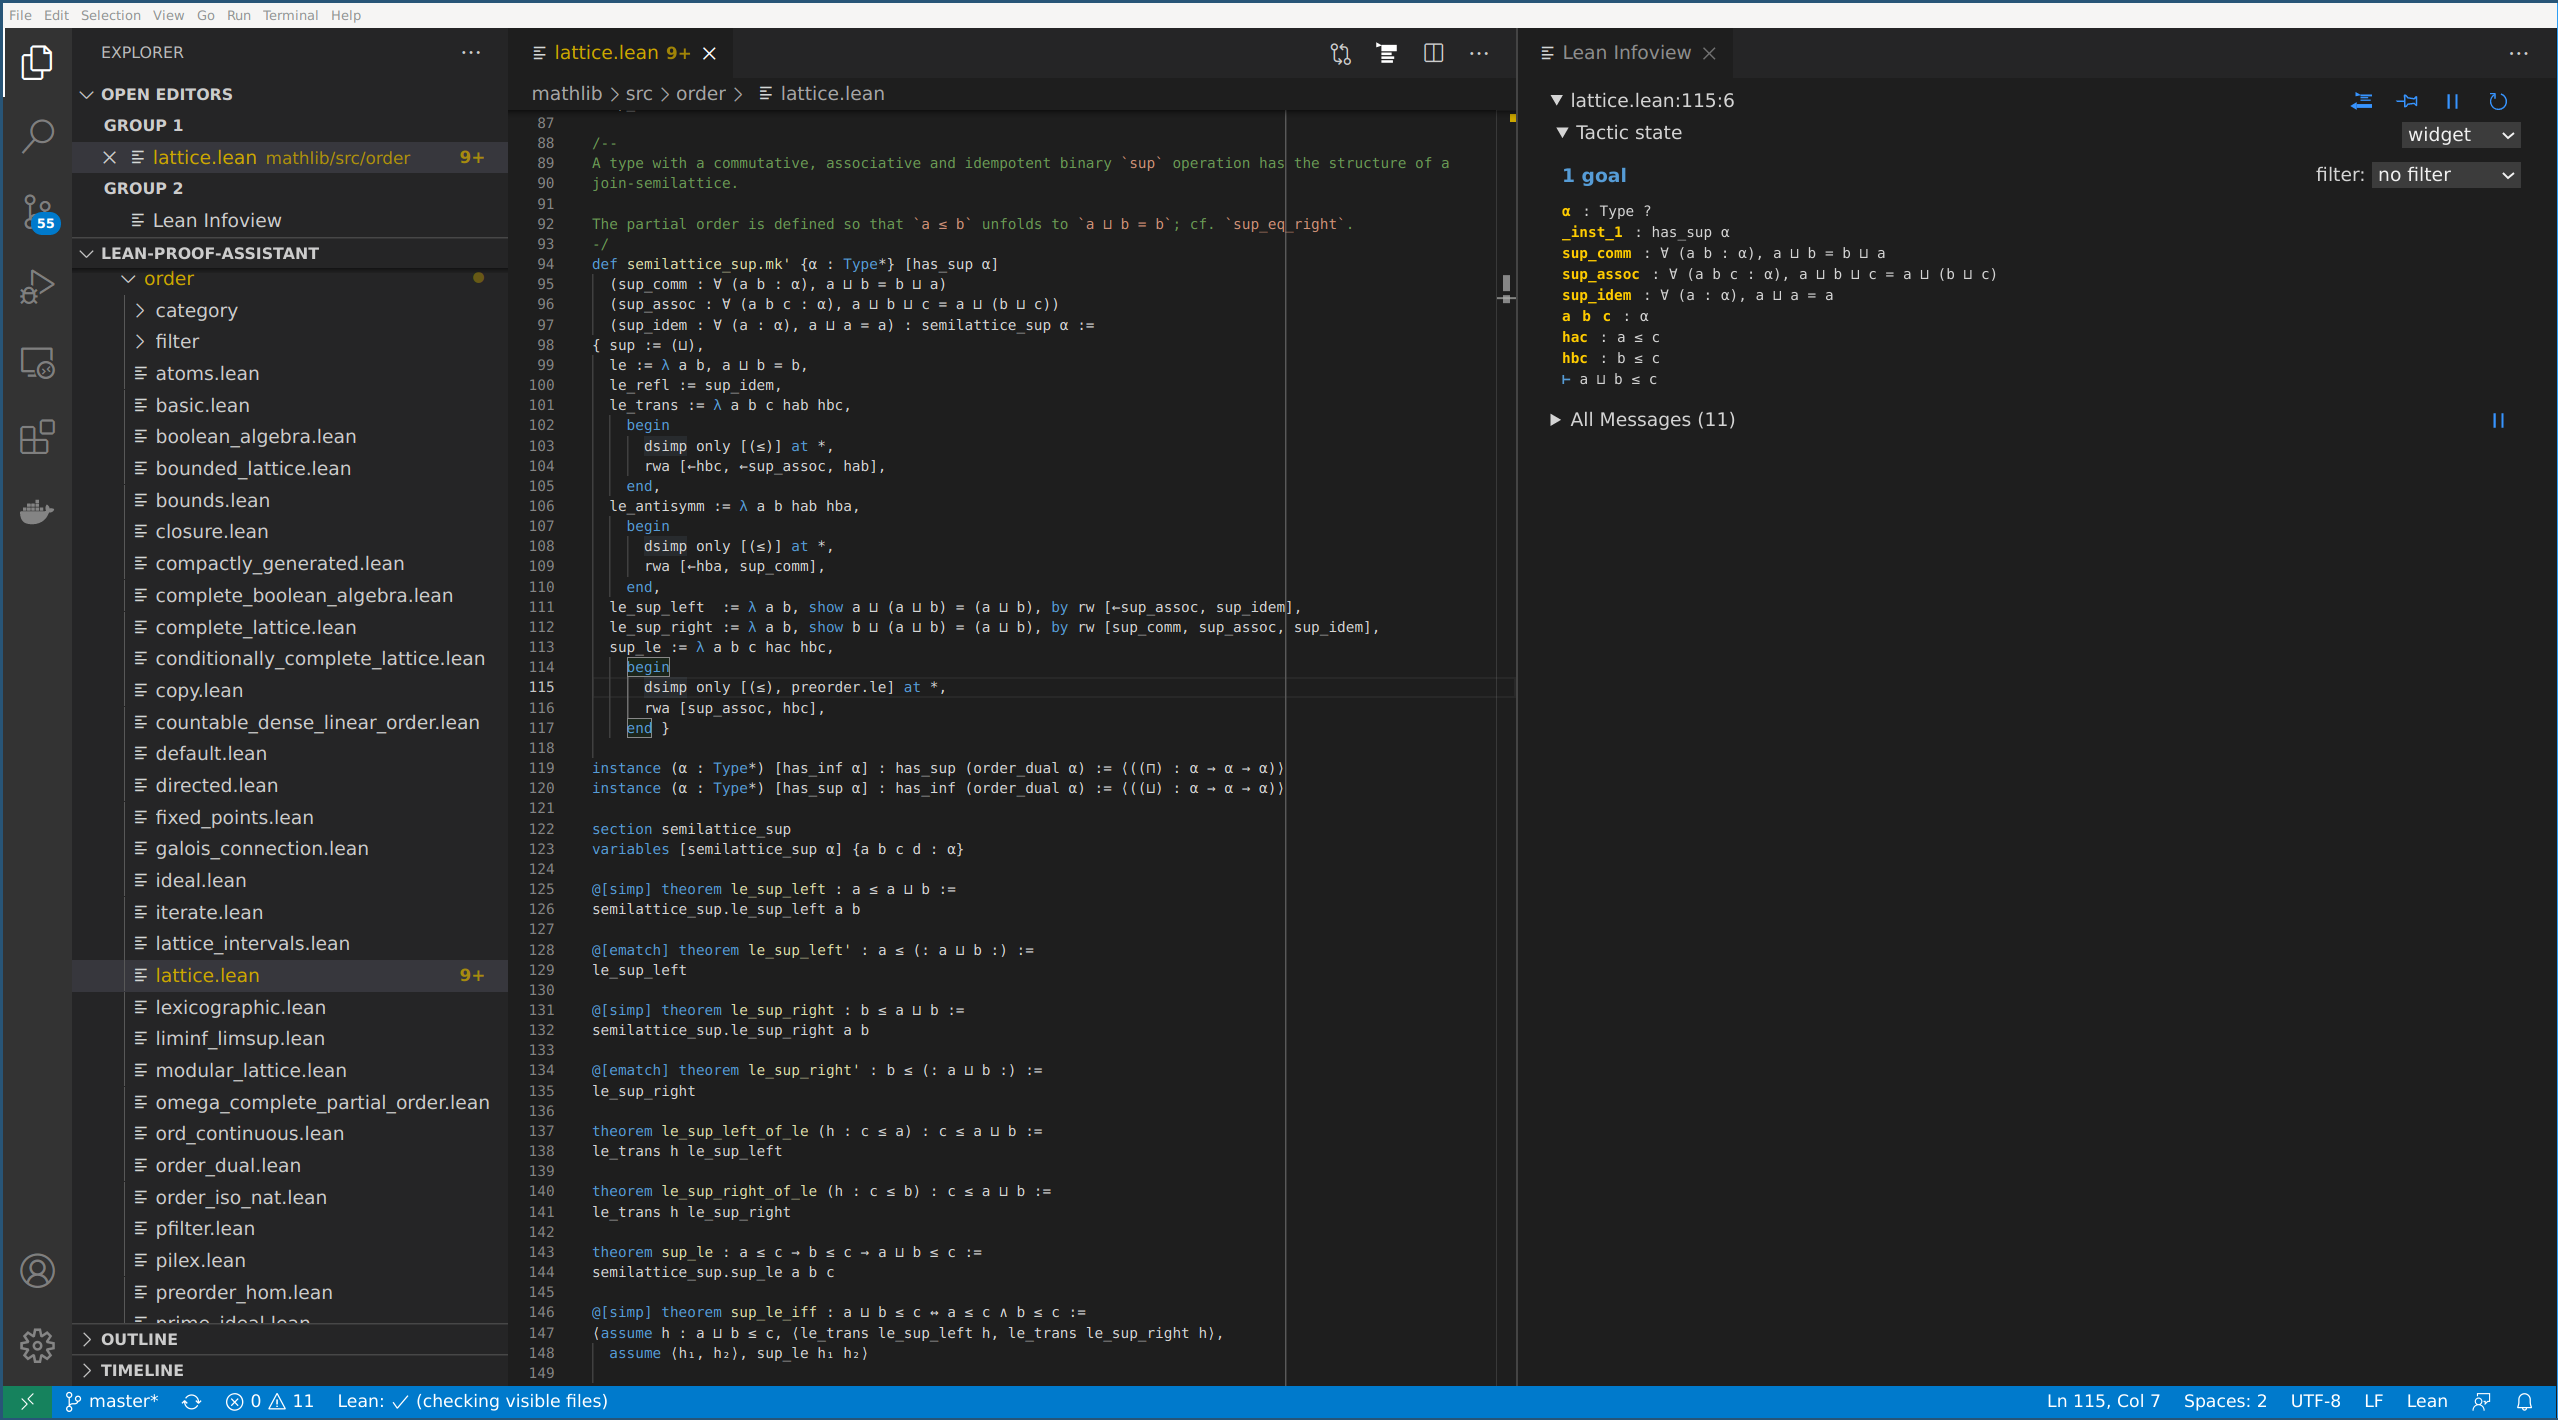
\includegraphics[scale=0.25]{vscode_printscreen.png}
        \caption{Vývojové prostredie}
    \end{figure}
\end{center}
    V pravom okne \emph{Lean infoview} je možné vidieť premenné s ich prislúchajúcimi
typmi a v prípade dôkazu aj formulu ktorú je potrebné dokázať za znakom $\vdash$.
    Okrem toho poskytuje okno aj výstup zo zabudovaných príkazov prostredia
ako \emph{print} alebo \emph{reduce} ktoré rozoberieme neskôr.
    V prípade že sa nachádzame v taktickom móde okrem zavedenia nových predpokladov
alebo transormácie existujúcich je možné vidieť aj zmenu cieľa a podcieľov
napríklad v prípade že sme sa dostali k dôkazu vymenovaním prípadov.
\section{Lambda kalkulus}
Pred predstavením techník dokazovania je nutné sa oboznámiť s prvkami funkcionionálneho
    programovania v Leane.
Výpočtový model jednoduchého $\lambda$-kalkulu je z programovacích paradigiem najbližšie
práve funkcionálnemu spôsobu programovania.
V nasledujúcej časti predstavujeme základy funkcionálneho programovania spolu
    s typmi a nástrojmi Lean-u na vývoj a menežment priestor mien.
\subsection{Konštanty, aplikácie}
    Deklarácia konštanty zavádza do systému novú deklaráciu bez definície.
    Z tohto dôvodu sa ich pri rozvoji teórie snažíme vyhýbať.
    V nasledujúcich príkladov budeme pracovať s prirodzenými a celými číslami
ktorých štruktúry sú súčasťou kontextu bez nutnosti ich importovať.
\begin{lstlisting}
constant m : nat
\end{lstlisting}
    Hovorí o deklarovaní konštanty $m$ ktorej typ je \emph{nat}.
    Alternatívny zápis pre prirodzené číslo je pomocou sekvencie \emph{\textbackslash nat}
alebo \emph{\textbackslash N} ktorú skonvertuje leanovské rozšírenie na znak $\mathbb{N}$.
    Vstavaný príkaz ktorý poskytuje typ výrazu zadaného na argumente je \emph{\#check}:
\begin{lstlisting}
#check m
\end{lstlisting}
    Mriežka na začiatku príkazu značí zabudovaný príkaz.
    V tomto prípade je to triviálne tak ako bola konštanta zadefinovaná s výstupom
v informačnom okne:
\begin{lstlisting}
m : ℕ
\end{lstlisting}
    Pre zadefinovanie viacerých konštánt jedným príkazom a nie len v tomto prípade
existuje plurárna verzia príkazu \emph{constants}.

    Definícia konštanty typu funkcie medzi prirodzenými číslami vyzerá nasledovne:
\begin{lstlisting}
constant f : ℕ → ℕ
constant h : ℕ -> ℕ -> ℕ
\end{lstlisting}
    Aplikácia funkcie sa notačne podobá aplikácii v $\lambda$kalkule kde argument
jednoducho pripíšeme za funkciu:
\begin{lstlisting}
#constants m n : ℕ

#check f m
#check h m
#check h m n
\end{lstlisting}
    Zatiaľ čo v prvom prípade dostaneme typ $\mathbb{N}$ v druhom prípade
$\mathbb{N} \to \mathbb{N}$ a v treťom vidíme aplikáciu na funkciu kde bude výsledným
typom znova jednoduchý typ $\mathbb{N}$.
    Aplikácia je asociatívna z ľavej strany a  preto je nasledujúci výraz potrebné 
ozátvorkovať napravo inak dostávame typový error pre funkciu $g$ ktorá očakáva 
celé číslo a nie typ funkcie f.
\begin{lstlisting}
constant f : ℕ → ℤ
constant g : ℤ → ℕ
constant a : ℕ

#check g (f a)
\end{lstlisting}
    Vo východiskovom prípade majú všetky čísla v editore typ $\mathbb{N}$.
\begin{lstlisting}
#check 5
#check (-5 : ℤ)
\end{lstlisting}
    Pri deklarácii záporného čísla je tak nutné už explicitne uviesť typ.
Nasledujúce príklady ilustrujú okrem funkcie $+$ aj implicitnú konverziu medzi typmi.
\begin{lstlisting}
#constants (m : ℕ) (n : ℤ)

#check 1 + 2
#check m + 1
#check n + 1
#check n + m
#check m + n
\end{lstlisting}
    V prípade prvého príkladu dostávame typ $\mathbb{N}$ pre nespracovaný výraz pre
ktorý by sme mohli očakávať výsledok $3$.
    Pre druhý a tretí výraz dostávame respektívne typy definovaných konštántých
premenných.
    Pri treťom výraze je vhodné si uvedomiť už implicitnú konverziu prirodzeného
čísla na celé.
    Konverzia je ešte viac zrejmá pri štvrtom výraze kde výsledným typom je
$\mathbb{Z}$.
    Prekvapivo z piateho výrazu dostávame v informačnom okne chybový výstup.
    Za neschopnosťou dostať typ stojí nedefinovaná konverzia z celých do prirodzených
čísel.
    Za vysvetlením stojí spôsob akým pracuje preťaženie infixového operátora $+$
podobným spôsobom ako pre triedy v jazyku $c++$ alebo $python$. Štvrtý a piaty
výraz je tak možné prepísať aj do tvaru:
\begin{lstlisting}
#check n.add(m)
#check m.add(n)
\end{lstlisting}
    Pretože znak $+$ je preťažením funkcie \emph{add} nad štruktúrou množiny daných
čísel.
\subsection{Abstrakcia}
    V predchádzajúcej sekcii sme si ukázali explicitný typ ktorý bol funkciou prirodzenými
číslami ktorý bol typu $\mathbb{N} \to \mathbb{N}$ alebo $\mathbb{N} \to \mathbb{N} \to \mathbb{N}$.
    V $\lambda$-kalklule zodpovedajú funkcie abstrakciám. V Lean-e definujeme
anonymnú funkciu alebo $\lambda$-výraz nasledovne.
\begin{lstlisting}
#check λ x, x + x
\end{lstlisting}
    Typ argumentu x je odvodený z výrazu ktorý na funkciu aplikujeme.
    Pre korektnú aplikáciu musí mať typ aj definovanú funkciu sčítania.
    Ak by sme chceli obmedziť argument len na konkrétny typ robíme to podobne ako
pri definovaní konštanty. Potom aplikácia
\begin{lstlisting}
#constant (m : ℤ)

#check (λ (x : ℕ), x + x) (m : ℤ)
\end{lstlisting}
je už typovou chybou pri ktorej nám informačné okno hlási
\begin{lstlisting}
type mismatch at application
  (λ (x : ℕ), x + x) m
term
  m
has type
  ℤ
but is expected to have type
  ℕ
\end{lstlisting}
    Uvedieme si zopár príkladov vypočtovo ekvivalentných funkcii obvodu obdĺžnika typu
$\mathbb{N} \to \mathbb{N} \to \mathbb{N}$
.
\begin{lstlisting}
#check λ x y, x + x + y + y
#check λ (x : ℕ) (y : ℕ), (x + x) + (y + y)
#check λ (x y : ℕ), (x + x) + (y + y)
#check λ (x : ℕ), λ (y : ℕ), (x + x) + (y + y)
\end{lstlisting}
    Zatiaľ čo prvý príklad je polymorfný a fungoval by aj pri aplikácii celých čísel,
nasledujúce sú ekvivalentné z pohľadu typov a predstavujú iný spôsob zápisu.

    V prípade že by sme chceli získať hodnotu z výrazu použíjeme príkaz \emph{\#eval},
alebo \emph{\#reduce}. \emph{Reduce} na rozdiel od \emph{eval} pri vykonávaní používa
jadro na získanie typu a je tak menej efektívnym.
\begin{lstlisting}
#eval (λ (x y : ℕ), (x + x) + (y + y)) 2 3
\end{lstlisting}
    Aplikácia nám dáva výsledok $10$ ktorý je očakávanou hodnotou.

    Pre pomenovanie alebo zadefinovanie takejto funkcie používame príkaz \emph{def}
ktorej tvar v najjednoduchšej podobe má tvar:
\begin{lstlisting}
def meno_definicie (argument_1 : typ) (argument_n : typ) :
    typ_navratovej_hodnoty 
:=
    telo funkcie
\end{lstlisting}
V prípade definície štvorca aj s jeho výpočtom
\begin{lstlisting}
def obvod_stvorca (x : ℕ) (y : ℕ) : ℕ := x + x + y + y

#eval obsah_stvorca 3 5
\end{lstlisting}

    Kľúčové slovo \emph{def} ktoré používame je funkčne bez funkčného roziedlu možné
zameniť za \emph{theorem}, \emph{lemma}. V prípade že chceme uviesť iba príklad
kde meno by pôsobilo nadbytočne používame slovo \emph{example}.

\subsection{Typy}
    Doteraz sme uvažovali len s typmi množiny prirodzených a celých čísel
predstavujúce na pozadí Leanu konkrétne definovanú štruktúru.
    Typovanie v Lean-e ale podporuje zavedenie nového abstraktného typu ktorý patrí univerzu(universe).
    Zavedenie týchto univerz je motivané problémom analogickým s Russelovým paradoxom 
a teda či množina všetkých množín obsahuje samú seba.
    V teórii typov sa jedná o Girardov paradox.
    Hierarchia týchto univerz je usporiadaná od 0 čo je univerzum tvoriace najjednoduchšie
typy takže \emph{Type} alebo aj \emph{Type 0} je potom typom \emph{Type 1} ktorý
je typom \emph{Type 2}.

    Špeciálne postavenie v typoch majú tvrdenia označujeme \emph{Prop}.
    Okrem toho že všetky dôkazy majú tento typ. 
    Sú postavené v hierachii oddelené na najnižšej úrovni a teda \emph{Prop} je 
typu \emph{Type}.
    Univerzum do ktorého patrí \emph{Prop} označujeme \emph{Sort} čo je len 
alias.
Platí vzťah \emph{Sort u + 1} = \emph{Type u}.

V tejto práci a ani vo väčšine práce s Leanom nie je potrebné využívať hierachiu
    typov sofistikovanejsie ako prezentovaným spôsobom.
\begin{lstlisting}
universe u v

constant (a : Typu u) (b : Type v)
\end{lstlisting}
Alebo je možné využiť substitučnú syntax kde \emph{*} znamená pre ľubovoľné univerzum
a v prípade \emph{\_} necháme doplniť typ automaticky Lean-om.
\begin{lstlisting}
constant f : Type _ → Type _
constant g : Type

#check f g
\end{lstlisting}
    Kontrola typu aplikácie nám vypíše typ \emph{Type u\_1} čo je spôsob Lean-u označovať
ešte neurčený typ bez konkrétneho univerza.
\subsection{Premenné}
    V prípade že sa snažíme definovať viacero funkcií s rovnakými arugmentami alebo
používať objekt ktorého typ je vyjadrený komplikovanejším zápisom je vhodné si
zápis zjednodušiť premennými.
    Z inak na pohľad komplikovaného zápisu
\begin{lstlisting}
universes u v

def kompozicia (α : Type u) (β : Type v) (f : α → β) (g : β → α) (x : α) :
    α
:=
    g (f x)

def kompozicia₂ (α : Type u) (β : Type v) (f : α → β) (g : β → α) (x : β) :
    β
:=
    f (g x)
\end{lstlisting}
    tak dostávame.
    Premenné vstupuju do predpokladov definícii len tam kde sú použíté v jej tele.
\begin{lstlisting}
universes u v

variables α : Type u
variables β : Type v

def kompozicia (x : α) (f : α → β) (g : β → α) : α := g (f x)
def kompozicia₂ (y : β) (f : α → β) (g : β → α) : β := f (g y)
\end{lstlisting}
    Vstupné argumenty dokonca môžeme vynechať úplne, v niektorých prípadoch to ale
môže byť kontraproduktívne.
\begin{lstlisting}
variables (f : α → β)
          (g : β → α)

def kompozicia : α := g (f x)
def kompozicia₂ : β := f (g y)
\end{lstlisting}
Pre doplnenie dodávame že nie je nutné ani definovať návratový typ $\alpha$
    respektíve $\beta$, explicitné určenie návratového typu je ale vhodné nie len
    pre čitateľa ale aj pre overenie správnosti výsledného typu.
\subsection{Kontext, priestor mien}
    Pre ovládanie menného priestoru a kontextu existujú v Lean-e rôzne mechanizmy
z ktorých si popíšeme len tie najdôležitejšie.
    Najjednoduchším je súbor, ktorého definície, konštanty a premenné vstupujú do
kontextu pri deklarácii a na konci súboru zaniknú.
    Import obsahu iných súborov sa robí jednoduchým príkazom \emph{import} ktorý
musí byť deklarovaný na začiatku súboru. V súborovej hierachii sa potom od najvyššej
úrovne v jednej z vyhľadávaných ciest vnorujeme cez bodku.
\begin{lstlisting}
import order.lattice
\end{lstlisting}
    Sa snaží nájsť priečinok \emph{order} so súborom \emph{lattice.lean}.
    V aktuálnej verzii Lean-u v čase písania práce sa dá zistiť zoznam prehľadávaných
ciest prepínačom \emph{path} priamo programu \emph{lean}.

    Deklarácie premenných definované v argumetnoch definície prepisujú vonkajší kontext.
    V prípade žeby sme chceli rozdeliť kontext súboru na menšie sekcie jednoduchým
nastrojom je dvojica \emph{section nazov\_sekcie}, \emph{end nazov\_sekcie}.
\begin{lstlisting}
section prirodzene_cisla
  variable α : ℕ
end prirodzene_cisla

section cele_cisla
  variable α : ℤ
end cele_cisla
\end{lstlisting}
    Používanejším je menný priestor \emph{namespace nazov} ktorý po zadefinovaní ponúka
možnosť opätovného zavedenia kontextu a vnorenie podobne ako rovnomenný mechanizmus
v jazyku C++.
\begin{lstlisting}
universe u

namespace skryty

  variable (α : Type u)
  namespace priestor
    def identita (a : α) : α := a
  end priestor
end skryty

#check skryty.priestor.identita

open skryty.priestor

#check identita
\end{lstlisting}
\section{Dokazovanie}

    K dokazovaniu v Leane je možné pristupovať viacerými spôsobmi.
    Po poskytnutí dôkazu už vnútorne Lean-u nezáleží na spôsobe akým bolo tvrdenie
dokázané.
    Prvým spôsobom je priamočiara konštrukcia typu pomocou funkcií.
    Druhým spôsobom je spätné dokazovanie ktoré využíva taktický mód za pomoci
sady príkazov poloautomatizácie.
    V leanovskej komunite je preferovaný práve druhý spôsob hoci pre jednoducho
dokázateľné tvrdenia stačí a je využívaná aj dopredná verzia.

\subsection{Dopredné dokazovanie}
    Dôkaz zostavený len z $\lambda$-funkcií ktoré transformujú argumenty
na výsledný typ je pri zložitejších dôkazoch ťažko čitateľný.
    Pre lepšiu čitateľnosť poskytuje Lean nástroje ktoré sa snažia konštruovať dôkazy tak
aby boli čitateľné ako tie klasické.
\begin{lstlisting}
variables p d : Prop

def plati_predpoklad : p → d → p := λ hp : p, λ hd : d, hp
\end{lstlisting}
    Predchádzajúci príklad je možné prepísať do čitateľnejšej verzie
\begin{lstlisting}
def plati_predpoklad : p → d → p :=
  assume hp : p,
  assume hd : d,
  show p, from hp
\end{lstlisting}
Pre lepšiu predstavu toho čo sa deje na pozadí Lean poskytuje výstup:
\begin{lstlisting}
pq: Prop
hp: p
hq: q
⊢ p
\end{lstlisting}

    Definícia hovorí o triviálnom tvrdení ak z $p$ vyplýva $d$ tak platí $p$. Voľným
prekladom sa dá dôkaz čítať ako:

\begin{itemize}
    \item Predpokladajme hp,
    \item a predpokladajme hd,
    \item potom vieme ukázať že platí p z predpokladu hp.
\end{itemize}

    O čosi zložitejším príkladom je tvrdenie že ak platí $p$ konjukcia $q$ tak potom
platí $q$ konjukcia $p$.

\begin{lstlisting}
def symetria_konjukcie : p ∧ q → q ∧ p :=
  assume hpq : p ∧ q,
    have hp   : p     := and.left  hpq,
    have hq   : q     := and.right hpq,
    have hqp  : q ∧ p := and.intro hq hp,
  show q ∧ p, from hqp
\end{lstlisting}

    Konjukciu v editore je možné napísať cez \emph{\textbackslash and}.
    Ak sa pozrieme na typ konjukcie a funkcií ktoré sme dostali cez príkaz check.
    Dostaneme výstup:

\begin{lstlisting}
and : Prop → Prop → Prop
and.left : ?M_1 ∧ ?M_2 → ?M_1
and.right : ?M_1 ∧ ?M_2 → ?M_2
and.intro : ?M_1 → ?M_2 → ?M_1 ∧ ?M_2
\end{lstlisting}

    Čo intuitívne korenšponduje s tým čo od týchto funkcií očakávame.
    Tento dôkaz je rozšírení o príkaz have ktorý vytvára predpoklad z existujúcich.
    V poslednej fáze dôkazu je interaktívny výstup:

\begin{lstlisting}
pq: Prop
hpq: p ∧ q
hp: p
hq: q
hqp: q ∧ p
⊢ q ∧ p
\end{lstlisting}

\subsection{Spätné dokazovanie}

V doprednom dokazovaní sme sa snažili transformovať predpoklady tak aby na konci
    bol výsledkom dôsledok.
Ako evokuje názov v spätnom dokazovaní sa snažíme transformovať cieľ tak aby sme
    sa dostali k jednému z predpokladov.
Pre tento účel existuje v Lean-e špeciálny spôsob dokazovania ktorý nazývame taktický
    mód.
Na rozdiel od dopredného dokazovania je nutné ovládať väčšiu sadu príkazov ktoré
    priamo transformujú cieľ.
Dokazovanie je tak užšie prepojené s interaktívnym prostredím a pripomína tak hru.
Ďalšou výhodou tohto dokazovania je možnosť využitie umelej inteligencie pri vyhľadaní
dôkazu.
Takýto prístup je obzvlášť užitočný napríklad v prípade že musíme dokázať identitu
    ktorej dôkaz je prácny, a tvorí ho veľa za sebou nasledujúcich využití iných
    identít ako napríklad využitie komutativity alebo asociativity.
Užšie prepojenie s prostredím a automatizácia vyhľadania dôkazu tohto módu ale
    ide na úkor priamej čitateľnosti.
Pre úplnosť doplňame že v taktickom móde nie je nutné transformovať cieľ a je možné
    využiť aj konštrukcie dopredného dôkazu.

Pre dokazovanie v taktickom móde používame konštrukciue ktorá je ohraničená
    konštrukciou \emph{begin} a \emph{end}.

\begin{lstlisting}
def symetria_konjukcie : p ∧ q → q ∧ p :=
  begin
    intro h,
    cases h with p q,
    split,
    exact q,
    exact p
  end
\end{lstlisting}

Dôkaz začína zavedením predpokladu z implikácie k ostatným o ktorých tvrdíme že
    sú pravdivé príkazom \emph{intro} a rozdelením konjukcie príkazom \emph{cases}
    s argumentom zavedenej konjukcie a ich explicitným pomenovaním.
Výstup z informačnom okne potom obsahuje.

\begin{lstlisting}
pq: Prop
p: p
q: q
⊢ q ∧ p
\end{lstlisting}

Príkazom \emph{split} potom rozdelíme cieľ na podciele kde sa snažíme dokázať
ľavú a pravú stranu ktorú vidíme v informačnom okne ako:

\begin{lstlisting}
2 goals
pq: Prop
h_left: p
h_right: q
⊢ q
pq: Prop
h_left: p
h_right: q
⊢ p
\end{lstlisting}

Dôkaz potom uzatvoríme príkazom \emph{exact} ktorý ukáže na jeden z predpokladov
    s rovnakým typom ako cieľ.

\section{Abstraktné štruktúry v Lean-e}
    V matematike a tak isto aj v programovaní sa často vyskytujú objetkov
nad ktorými je možné vykonávať operácie bez ohľadu na ich obsah pri splnení
určitých podmienok.
    V matematike hovoríme o štruktúrach ktoré majú striktnú definíciu v programovaní
sa dá voľne hovoriť o triedach.
    Matematické štruktúry v Lean-e su navrhované práve pomocou mechanizmu tried.
    Kde definícii triedy zodpovedá štruktúra spĺňajúca z definíce vyplývajúce podmienky.
    Potom inštanciou triedy môže byť znova štruktúra ktorá je definovaná na užšej množine
znova spĺňajúcej podmienky, príkladom je vzťah grupy a podgrupy alebo
priestoru a podpriestoru.
    Alebo iná množina ktorá spĺňa okrem podmienok pôvodnej štruktúry ďalšie ktoré ju
obohacujú.
    Príkladom takého vzťahu môže byť pologrupa ktorý je množinou s asociatívnou operáciou
a pologrupou ktorá má aj neutrálny prvok.

\subsection{Induktívne štruktúry}

    Induktívne štruktúry predstavujú notačne silný nástroj pre definíciu objektov
ktorých prepojenia medzi prvkami sú prepojené jednoduchou asociáciou.
    Jednoduchým príkladom je zoznam kde asociáciou medzi prvkami tvorí vzťah
usporiadania.
    Komplikovanejší klasický príklad tvoria stromové štruktúry tvoriace uzly
s viacerými nasledovníkmi patriace jednému uzlu.
    V matematike sa s indukciou stretávame pri definícii prirodzených čísel
cez Peanove axiómy.
    Dve z týchto axióm hovoria:
\begin{itemize}
    \item 0 je číslo
    \item Ak $a$ je číslo potom nasledovník $a$ je tiež číslo.
\end{itemize}
    Prvé pravidlo hovorí o základnom prípade, v prípade zoznamu alebo stromu prázdny
zoznam respektíve strom.
    Implementácia prirodzených čísel pomocou indukčnej štruktúry by mohla vyzerať
nasledovne:
\begin{lstlisting}
inductive prirodzene : Type
  | nula        : prirodzene
  | nasledovnik : prirodzene → prirodzene
\end{lstlisting}
    Za kľúčovým slovom inductive nasleduje názov a sada konštruktorov s návratovými
typmi.
    Už z názvu vyplýva súvislosť s dôkazom s matematickou indukciou kde platnosť
nejakého tvrdenia $P(n)$ pre všetky prirodzené čísla sa dokazuje pre
\begin{itemize}
    \item $P(0)$, t.j. základný prípad
    \item $\forall n \in \mathbb{N}, P(n) \implies P(n+1)$, indukčný krok
\end{itemize}
    Pre tento typ dôkazu existuje v Leane v taktickom móde príkaz \emph{induction}.
\begin{lstlisting}
example : 5 * n = 4 * n + n :=
    begin
      induction n with d hd,
      ...
    end
\end{lstlisting}
    Po príkaze induction sa informačnom nachádzaju dva ciele pre obe konštruktory
prirodzených čísel \emph{nat.zero} a \emph{nat.succ} podobne ako v našej uvedenej
štruktúre a základnemu prípadu a tvrdeniam matematickej indukcie dokazujúcej platnosť
$P$.
\begin{lstlisting}
case nat.zero
⊢ 5 * 0 = 4 * 0 + 0

case nat.succ
d: ℕ
hd: 5 * d = 4 * d + d
⊢ 5 * d.succ = 4 * d.succ + d.succ
\end{lstlisting}

    V príklade ktorý sme uviedli sú znamienká $+$ a $*$ ktoré používame
v operáciach nad typom našej induktívnej štruktúry.
    Výsledkom oboch binárnych operácii je znova prirodzené číslo.
    Podľa predpokladov typ ktorý prislúcha ich definícii je
$prirodzene \to prirodzene \to prirodzene$.
    Jednou z výhod indkučne definovaných štruktúr je jednoduchosť definovania
rekurzívnych funkcií ktoré operujú nad týmito štruktúrami.
\begin{lstlisting}
variables (a b: prirodzene)

open prirodzene

def sucet : prirodzene → prirodzene → prirodzene
  | a    nula         := a
  | a (nasledovnik b) := nasledovnik (sucet a b)
\end{lstlisting}
    V tomto prípade znamená notácia $|$ prípad v ktorom sa snažíme nájsť zhodu
s poskytnutým arugmentom a návratový typ.
    V treťom prípade ide o rekurzívne pravidlo ktoré z argumentu $b$ vytvorí jedo
predchodcu.
    Celé pravidlo potom vráti nasledovníka zo súčtu prvého argumentu a predchodcu
druhého.
    Rekurzia tak prenáša vlastnosť nasledovania z prvého na druhý argument až
sa argumenty nezhodujú s prvým pravidlom a teda argument už nemá predchodcu.
    Pre úplnosť dodávame aj technický detail definovania znamienka $+$ ako volania
funkcie súčtu:
\begin{lstlisting}
local infix ` + ` := sucet
\end{lstlisting}

\subsection{Jednoduché štruktúry}
    V prípade že by jeden z konštruktorov neobsahoval typ ktorý poskytuje funkciu
medzi typmi samotnej štruktúry, ide o obyčajnú štruktúru.
    Ich využitie je najmä pri definovaní tých matematických a v lean-e majú
špeciálnu syntax.
    V príklade uvádzame ekvivalentné spôsoby definovania štruktúr.
\begin{lstlisting}
structure vector :=
  mk :: (x y: ℕ)

structure vector₂ :=
  (x : ℤ)
  (y : ℤ)
\end{lstlisting}
    Vytváranie objektov danej štruktúry má explicitné priradzovanie prvkom
podľa názvov v prípade jednoduchých štruktúr je vhodnejšie priradzovanie na
základe poriadia z definície šturktúry.
\begin{lstlisting}
def v₂ : vector₂ :=
  {
    x := 10,
    y := 20,
  }

#check (⟨10, 20⟩ : vector)
\end{lstlisting}
    K jednotlivým prvkom štruktúry pristupujeme cez bodku:
\begin{lstlisting}
#eval v.x
\end{lstlisting}
    tak vracia hodnotu 10.
    Pre modelovanie hierarchie kde jedna štrutúra rozširuje druhú používame
kľúčové slovo \emph{extends}.
    Rozšírenie našej štruktúry o ďalšiu dimenziu vyzerá nasledovne:
\begin{lstlisting}
structure vector₃ extends vector₂ :=
  (z : ℤ)

def ∨₃₁ : vector₃ :=
  { x := 1, y := 2, z := 3}
\end{lstlisting}
    V prípade že chceme vytvoriť objekt z rošírenej štruktúry a máme k dispozícii
jeho podkladový je častov využívaná notácia.
\begin{lstlisting}
def ∨₃₂ : vector₃ :=
{
    z := 10, ..v₂
}
\end{lstlisting}

Tu ešte vysvetlím závistlostné typy.

\subsection{Typové triedy}
    Typové triedy poskytujú mechanizmus pomocou ktorého zlučujeme rozdielnym štruktúram
s rovnakou vlastnosťou do tried.
    Príkladom môžu byť mať vlastnosť usporiadania, štruktúra má reprezentanta alebo
je grupou.
    Po zadefinovaní triedy potom štruktúru priradíme do tried inštancovaním.
    Inštancovanie pre štruktúry potom býva odlišné v závislosti definície štruktúry.
    Vykonávanie dôkazov nad typovou triedou potom umožňuje zredukovať množstvo definícii.
    Nad našimi definíciami vektorov môžeme definovať dĺžku.
\begin{lstlisting}
class length (α : Type u) :=
  (length : α → ℝ)
\end{lstlisting}
    Potom k definíciam štruktúr pridáme inštancie.
\begin{lstlisting}
instance vector₂_length : length vector₂ :=
 { length := λ (v : vector₂), sqrt(v.x * v.x + v.y * v.y) }

instance vecotr₃_length : length vector₃ :=
 { length := λ (v : vector₃), sqrt(v.x * v.x + v.y * v.y + v.z * v.z) }
\end{lstlisting}
    Triedu potom využívame v definíciach uvedením do hranatých zátvoriek aj s
argumentom.
\begin{lstlisting}
def meno_definicie (argument : Type) [ dlzka argument ] : Type :=
begin
    ...
end
\end{lstlisting}

Kód som ešte neskontroloval pretože mi hapruje Lean.

\chapter{Teória usporiadania}
    V tejto kapitole sa budeme snažiť ukázať možnosti Lean-u a využitie už existujúcich
definícii v mathlibe pre dokázanie viet týkajúcich sa teórie usporiadania.
    Pre tento účel je Lean ideálny z pohľadu našich možností definovania vlastností
usporiadania, ktoré následne možno aplikovať na abstraktnú množinu objektov.
    % Toto by bolo dobré rozpracovať ďalej, možno konkrétny príklad
    Výsledný typ je potom odvodený na základe závislostných typov.
    Usporiadanie je jednoducho intuitívne uchopiteľná vlastnosť bez matematických
preddispozícií.
    V každodennom živote porovnávame svoju výšku, čas, ktorý trval na vybehnutie do kopca
alebo aj číselne neohodnotené, subjektívne merateľné objekty ako ktorý album
od skupiny preferujem.
    Na otázky si potom vieme odpovedať "ja som vyšší", "zabehol si pomalšie" alebo
tieto albumy sú neporovnateľné.

Teória usporiadania sa snaží tieto vlastnoti formálne definovať a rozvíjať ďalej
otázkami ako, aké je horné celej množiny objektov. Existuje ohraničenie horné alebo
dolné pre ľubovoľnú podmnožinu objektov?
    Pre stručnosť sa v rámcii definícii obmedzíme len na definíciu usporiadania
ako relácie, čiže podmnožinu karteziánskeho súčinu dvoch množín.

\begin{theorem}
    Majme množinu $P$, potom usporiadanie alebo čiastočné usporiadanie na množine
    $P$ je binárna relácia $\leq$ taká že, pre všetky $x,y,z \in P$
    \begin{itemize}
        \item $x \leq x$ vlastnoť reflexivity
        \item $x \leq y$ a $y \leq x$ implikuje $x = y$ antisymetria
        \item $x \leq y$ a $y \leq z$ impikuje $x \leq z$ tranzitivita
    \end{itemize}
\end{theorem}

    Ideálnym nástrojom pre uvažovanie nad usporiadaním sú \emph{Hasseho} diagramy.
    Ako príklad uvádzame diagram "kocky".

\begin{figure}[!ht]
    \centering
    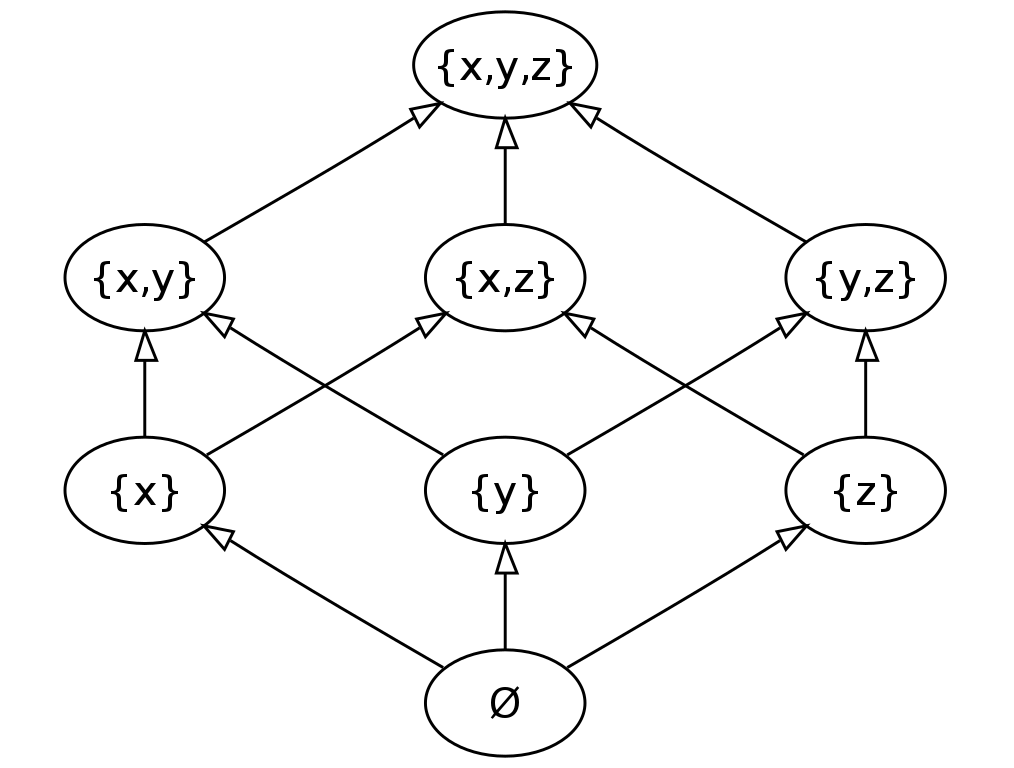
\includegraphics[scale=0.15]{cube.png}
    \caption{Usporiadania $\mathcal{P}(\{a,b,c\})$}
\end{figure}

    Na obrázku je usporiadanie všetkých podmnožín trojprvkovej množiny $\{ a,b,c \}$.
    Usporiadanie tvorí binárna relácia kardinality podmnožínm pričom porovnávame
len podmnožiny obsahujúce spoločný prvok.
    Vyššie sú položené väčšie prvky a porovnateľnými prvkami považujeme len tie,
ktoré sú "pokryté" jednosmernou cestou cez orientované hrany grafu.

    V Leane je usporiadanie definované ako rozšírenie triedy predusporiadania, ktorá
je reláciou, ktorá nemá oproti čiastočnému usporiadaniu vlastnosť antisymetrie.

\begin{lstlisting}
class has_le       (α : Type u) := (le : α → α → Prop)
class has_lt       (α : Type u) := (lt : α → α → Prop)

class preorder (α : Type u) extends has_le α, has_lt α :=
(le_refl : ∀ a : α, a ≤ a)
(le_trans : ∀ a b c : α, a ≤ b → b ≤ c → a ≤ c)
(lt := λ a b, a ≤ b ∧ ¬ b ≤ a)
(lt_iff_le_not_le : ∀ a b : α, a < b ↔ (a ≤ b ∧ ¬ b ≤ a) . order_laws_tac) -- toto chceme aj vysvetlit
\end{lstlisting}
Čiastočné usporiadanie je potom rozšírením predusporiadania o vlastnosť antysymetrie.
\begin{lstlisting}
class partial_order (α : Type u) extends preorder α :=
(le_antisymm : ∀ a b : α, a ≤ b → b ≤ a → a = b)
\end{lstlisting}

DOPLN PRIKLAD NAJLEPSIE AK NAS USPORIADANY POSET Z PRIKLADU

\subsubsection{Zväz}
    Zväz je usporiadaná množina, pre ktorú navyše platí, že pre každé 2 prvky $a, b$
vieme nájsť prvok $c$, ktorý je ich jedinečným najmenším horným, respektíve(\emph{supremum})
najväčším dolným ohraničením(\emph{infinum}).
    V prípade intervalu reálnych čísel je toto ohraničenie jednoducho predstaviteľné
ako bod ohraničujúce množinu na číselnej osi.
    Ak ide o čiastočné usporiadanie, názov je pre tieto ohraničenia prvkov
motivovaný zobrezním na grafe.
    \emph{Spojenie} $\sqcup, \vee$ pre supremum, respektíve \emph{priesek} $\sqcap, \wedge$ pre infinum.
    Popisnejším názvom pre zväz je preklad anglicky používaného názvu \emph{lattice}
"mriežka" tak isto motivovaná zobrazením takého usporiadania na grafe.
    Pri dokazovaní viet o zväzoch je často využívaná vlastnosť duality najmenšieho
horného a duálne najväčšieho dolného ohraničenie pre druhú polovicu dôkazu.
    V prípade zväzu je táto vlastnosť využitá rovno v definícii zväzu ako spojenie
duálnej definície suprémoveho a infinumového semizväzvu.

\begin{lstlisting}
class has_sup (α : Type u) := (sup : α → α → α)
class has_inf (α : Type u) := (inf : α → α → α)

infix ⊔ := has_sup.sup
infix ⊓ := has_inf.inf

class semilattice_sup (α : Type u) extends has_sup α, partial_order α :=
(le_sup_left : ∀ a b : α, a ≤ a ⊔ b)
(le_sup_right : ∀ a b : α, b ≤ a ⊔ b)
(sup_le : ∀ a b c : α, a ≤ c → b ≤ c → a ⊔ b ≤ c)

class semilattice_inf (α : Type u) extends has_inf α, partial_order α :=
(inf_le_left : ∀ a b : α, a ⊓ b ≤ a)
(inf_le_right : ∀ a b : α, a ⊓ b ≤ b)
(le_inf : ∀ a b c : α, a ≤ b → a ≤ c → a ≤ b ⊓ c)

class lattice (α : Type u) extends semilattice_sup α, semilattice_inf α
\end{lstlisting}

Na nasledujúcich grafoch si ukážeme ako vyzerajú zväzy.

PRIDAT VLASTNY PRIKLAD, OPYTAT SA
\begin{lstlisting}
def poset_nat : sublattice ℕ :=
    { carrier := {n : ℕ | 1 ≤ n},
    inf_mem :=
      begin·
        intro a,
        intro b,
        intro a_set,
        intro b_set,
        simp at a_set,
        simp at b_set,
        simp,
        split,
        exact a_set,
        exact b_set,
      end,
    sup_mem := by finish,
}
\end{lstlisting}

\subsubsection{Modulárne zväzy}

V nasledujúcom úseku si ukážeme vetu týkajúcu sa špeciálneho typu zväzu s vlastnosťou
    modularity a ukážeme si formálny dôkaz a jej implementáciu v Leane, ktorú si
    podrobne rozoberieme.

O zväze $L$ hovoríme, že je modulárny, v prípade, že má nasledujúcu vlastnosť.

\begin{equation*}
    (\forall x,y,z \in L) x \geq y \implies x \wedge ( y \vee z) = (x \wedge y) \vee z
\end{equation*}

V Leane definovaný ako rozšírenie zväzu:

\begin{lstlisting}
class modular_lattice(α : Type u) extends lattice α :=
  (modular_law: ∀ (x u v : α ), (x ≤ u) → u ⊓ (v ⊔ x) = (u ⊓ v) ⊔ x )
\end{lstlisting}

V nasledujúcom úseku si ukážeme vetu o modulárnom izomorfizme a podrobne
    si rozoberieme implementáciu jej dôkazu s obsahom prostredia v Leane.

TODO ZJEDNOTIT ZNACENIE DEFINICIE A LEAN-u
\subsection{Modulárne zväzy}
    \begin{theorem} \emph{Veta o izomorfizme modulárnych zväzov}
    Nech L je modulárnym zväzom a $a, b \in L$. Potom
        \begin{equation}
            \varphi_{b}: x \mapsto x \wedge b, x \in [a, a \vee b],
        \end{equation}
    Je izomorfizmom medzi intervalmi $[a, a \vee b]$ a $[ a \wedge b, b]$.
    Inverzným izomorfizmom je
        \begin{equation}
            \psi_{a}: y \mapsto x \vee a, y \in [a \wedge b, b].
        \end{equation}
    \end{theorem}
    \emph{Dôkaz}.  Stačí ukázať, že $\varphi_{b}\psi_{a}(y) = y$ pre všetky $x \in [a, a \vee b]$.
    Z duality vyplýva, že $\varphi_{b}\psi_{a}(y) = y$ pre všetky
        $y \in [a \wedge b, b]$,
    Majme $x \in [a, a \vee b]$. Potom
        $\psi_{a}\varphi_{b} = ( x \wedge b ) \vee a$ nerovnosť $a \leq x$ platí
        potom aj modularita
        \begin{equation}
            \varphi_{a}\psi_{b}(x) =
            ( x \wedge b ) \vee a =
            x \wedge ( b \vee a) =
            x
        \end{equation}
        pretože
        \[
            \pushQED{\qed}
            x \leq a \vee b. \qedhere
            \popQED
        \]

    Predstavený dôkaz je znázornený na nasledujúcom grafe.

\begin{figure}[!ht]
    \centering
    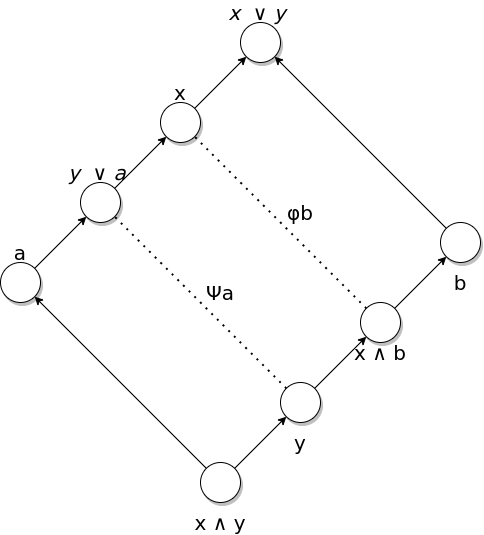
\includegraphics[scale=0.35]{modular_lattice_isomorphism.png}
    \caption{Izomorfizmus modulárneho zväzu}
\end{figure}

    V prípade formálneho dôkazu sme sa mohli v časti dôkazu odkázať na dualitu. 
    V prí návrhu dôkazu v Leane musíme ukázať dôkaz z "oboch" strán.

\begin{lstlisting}
theorem modular_lattice_isomorphism { α: Type u } [ modular_lattice α ]
{ u v w x y : α } :
  x ≤ u →
  x ≥ v →
  x ≥ u ⊓ v →
  x ≤ u ⊔ v →
  u ⊓ ( v ⊔ x ) = x ∧ (u ⊓ x) ⊔ v = x
  :=
  begin
 1        intros h1 h2 h3 h4,
 2        split,
 3        {
 4          rw modular_lattice.modular_law,
 5          exact sup_eq_right.mpr h3,
 6          exact h1
 7        },
 8        {
 9          rw inf_comm,
10          rw ← modular_lattice.modular_law,
11          exact inf_eq_left.mpr h4,
11          exact h2
12        }
  end
\end{lstlisting}
    Začíname v taktickom móde prázdnou konštrukciou \emph{begin} a \emph{end}
    Interaktívne prostredie vyzerá nasledovne.
\begin{lstlisting}
α: Type u
_inst_1: modular_lattice α
u v w x y : α
⊢ x ≤ u → x ≥ v → x ≥ u ⊓ v → x ≤ u ⊔ v → u ⊓ (v ⊔ x) = x ∧ u ⊓ x ⊔ v = x
\end{lstlisting}
    Prvým krokom dôkazu je presunutie predpokladov zo sledu implikácii do
prostredia pre ďalšiu prácu s nimi s označením $h1,h2,h3,h4$.
\begin{lstlisting}
α: Type u
_inst_1: modular_lattice α
uvwxy: α
h1: x ≤ u
h2: x ≥ v
h3: x ≥ u ⊓ v
h4: x ≤ u ⊔ v
⊢ u ⊓ (v ⊔ x) = x ∧ u ⊓ x ⊔ v = x
\end{lstlisting}
    Cieľ potom pozostáva z konjukcie, kde v druhej časti máme výraz implicitne
ozátvorkovaný zľava.
    Výraz rozdelíme do dvoch podcieľov príkazom \emph{split}, a pre lepšiu
čitateľnosť ozátvorkujeme množinovými zátvorkami. Nachádzame sa v stave
\begin{lstlisting}
  begin
    intros h1 h2 h3 h4,
    split,
    {
    },
    {
    }
  end
\end{lstlisting}
v ktorom nám lean ukazuje prostredie, kde musíme dokázať ľavú časť konjukcie.
\begin{lstlisting}
⊢ u ⊓ (v ⊔ x) = x
\end{lstlisting}
Na cieľ použijeme z definície modulárneho zväzu vlastnosť modularity
\begin{lstlisting}
    (modular_law: ∀ (x u v : α ), (x ≤ u) → u ⊓ (v ⊔ x) = (u ⊓ v) ⊔ x )
\end{lstlisting}
a transformujeme prepíšeme cieľ cez príkaz
\begin{lstlisting}
rw modular_lattice.modular_law,
\end{lstlisting}
na nasledujúci, kde má $u \sqcap v$ vyššiu precedenciu
\begin{lstlisting}
⊢ u ⊓ v ⊔ x = x
\end{lstlisting}
    Nasledujúca transformácia vyžaduje znalosť už dokázaných definícií, ktoré
boli dokázané pre podkladové štruktúry. Použijeme nasledujúcu definíciu, ktorá vychádza
z kontextu \emph{semilattice\_sup}.
\begin{lstlisting}
% @[simp] theorem sup_eq_right : a ⊔ b = b ↔ a ≤ b :=    / TODO NEZABUDNUT
%  le_antisymm_iff.trans $ by simp [le_refl]             / ODKOMENTOVAT
    \end{lstlisting}
    Zaujímavosťou je, že si Lean dokáže substiuovať výraz $u \sqcap v$ za $a$ z uvedeného
výrazu. Pri použití vety dostávame ekvivalenciu, ktorá je definovaná ako štruktúra.
\begin{lstlisting}
structure iff (a b : Prop) : Prop :=
    intro :: (mp : a → b)
             (mpr : b → a)
\end{lstlisting}
Z tejto štruktúry použijeme implikáciu smerujúca doľava nasledovne:
\begin{lstlisting}
    exact sup_eq_right.mpr h3,
\end{lstlisting}
    Cieľ je teda transformovaný na:
\begin{lstlisting}
⊢ x ≤ u
\end{lstlisting}
čo je už uvedený predpoklad $h1$. Týmto sme dokázali jeden z podcieľov.
    V tejto chvíli by sme sa v literatúre mohli odvolať na dualitu výrazov.
    V Leane musíme poskytnúť dôkaz aj o druhom cieli. Ideme dokázať
\begin{lstlisting}
⊢ u ⊓ x ⊔ v = x
\end{lstlisting}
V tejto chvíli chceme znova použiť modularitu, leanu je, ale potrebné explicitne povedať,
    že chceme prepísať výraz nachádzajúci na pravej strane rovnosti pomocou symbolu
ľavej šípky.
\begin{lstlisting}
rw ← modular_lattice.modular_law,
\end{lstlisting}
    Použijeme duálnu vetu
    duálnu k \emph{sup\_eq\_right}.
\begin{lstlisting}
@[simp] theorem inf_eq_left : a ⊓ b = a ↔ a ≤ b
\end{lstlisting}
    a využijeme opačné predpoklady k predchádzajúcim $h2, h4$.
\begin{lstlisting}
{
    rw ← modular_lattice.modular_law,
    exact inf_eq_left.mpr h4,
    exact h2
}
\end{lstlisting}

Po dokázaní druhého cieľa sme dokázali celú vetu. $\square$

\begin{thebibliography}{xx}
    \bibitem{Mimram} Samuel Mimram, Program = Proof, Indenpendently published(July 3, 2020), ISBN-13: 979-8615591839
    \bibitem{SorensenUrzyczyn} Morten Heine B. Sørensen, Pawel Urzyczyn, Lectures on the Curry-Howard Isomorphism,
        Elsevier Science (April 4, 2013),  ISBN-13 : 978-0444545961
    \bibitem{lean3} https://github.com/leanprover/lean
    \bibitem{lean4} https://github.com/leanprover/lean4
    \bibitem{mathlib} https://github.com/leanprover-community/mathlib
    \bibitem{mathlib_paper} https://leanprover-community.github.io/papers/mathlib-paper.pdf
\end{thebibliography}

Slovicka na ktore nepoznam preklad a ne
\begin{itemize}
    \item kalkul alebob kalkulus
    \item namespace - priestor mien
    \item universe - univerzum
\end{itemize}

\end{document}

\begin{verbatim}
    structure point :=
      ( x : nat )
      ( y : nat )

    /-- alternative notation -/
    structure point_alternative :=
      mk :: (x : nat) (Y : nat)

    def p1 : point :=
    {
      x   := 10,
      y   := 20,
    }

    /- same point, different notation, same notation for ordered seti -/
    def p2 : point := $\langle 10, 20 \rangle$

    /- instance only one part of structure, rest implicitly from other instance
    def p3 : point := {
        x := 20,
        ..p
    }
\end{verbatim}

% sposob ukladania kodu

\subsubsection{Type classes}

